\documentclass[10pt,a4paper,DIV=15]{scrartcl}
\usepackage{ngerman}
\usepackage[latin1]{inputenc}
\usepackage[T1]{fontenc}
\usepackage{graphics}
\usepackage{graphicx}
\usepackage{subfigure}
\usepackage{amsmath}
\usepackage{amssymb}
\usepackage{mathcomp}
\usepackage{dsfont}
\usepackage[Algorithmus]{algorithm}
\usepackage{algorithmic}
\usepackage{url}
\usepackage[colorlinks,linkcolor=black,urlcolor=blue,citecolor=black]{hyperref}

\title{Vorlesung Multidimensionale und Multimodale Signale, SoSe 2010}
\author{Sebastian Rockel (6095961)\\Vitali Amann (5788408)}
\date{\today}

\begin{document}
\maketitle
%Loesung zum Uebungsblatt 1:
%\section*{1 �bung (Abgabe: 14.04.2010, 8.30 Uhr, schriftlich)}

\subsection*{1. Beschreiben Sie anschaulich den Begriff Frequenz anhand verschiedener Beispiele.}
Die Frequenz ist die H�ufigkeit eines sich regelm��ig wiederholenden Vorgangs. [wikipedia]\\
Frequenzen treten in unserer (Um-)Welt �berall auf. Beispielsweise hat der Strom aus unserer Steckdose eine Frequenz von 50 Herz, er schwingt also 50 mal in der Sekunde. Eine Schwingung fasst dabei den Vorgang zusammen, in dem die schwingende Gr��e wieder am Ausgangspunkt angelangt ist. Weitere sind z.B. Puls, Bildschirmwiederholfrequenz, Lichtspektrum, Schwingfrequenz von Atomen/Teilchen.\\
Jeder K�rper scheint eine Eigenfrequenz zu haben, in der er ``schwingtn''.

\subsection*{2. Sehen Sie einen Zusammenhang zwischen dem Begriff Frequenz und der folgenden Abbildung?}
Bilder kann man neben der ikonischen Ebene auch in der spektralen Ebene betrachten. Dabei sind hohe Frequenzen f�r die scharfen Anteile und niedrige f�r die verschwommenen zust�ndig. Entsprechend kann man ein Bild mittels Hochpass sch�rfen (tiefe Frequenzen werden gefiltert) und mittels Tiefpass weich zeichnen (hohe Frequenzen werden gesperrt).\\
Das Bild enth�lt hohe und tiefe Frequenzen von 2 urspr�nglich verschiedenen Bildern. Die scharfen Anteile geh�ren zu Albert Einstein, die unscharfen Marilyn Monroe.

\subsection*{3. Lesen Sie den Artikel auf der Seite XY und vergleichen Sie dies mit der obigen Abbildung.}
Die scharfen Gesichtskonturen der Mona Lisa zeigen kein L�cheln (bzw. wenig), die Unscharfen (Schatten der Gesichtspartien, bes. Wangen) zeigen eins.\\
Das menschliche Sehsystem kann scharfe Kanten im Fokus-Zentrum sehr gut erkennen, im �u�eren Sichtfeld werden dagegen nur unscharfe Objekte wahrgenommen.\\
Sieht man nun direkt auf den Mund �berwiegt dieser in der Wahrnehmung (nicht l�chelnd). Nimmt man dagegen das Gesicht im peripheren Sichtbereich war, �berwiegen die unscharfen Konturen (l�chelnd).

%Loesung zum Uebungsblatt 2:
%\section*{2 �bung (Abgabe: 22.04.2010, 8.30 Uhr, schriftlich)}

\subsection*{1. Gegeben sei eine periodische Funktion �ber die Zeit, wie lauten die Fourierkoeffizienten?}
a) $f(t) = \sin(t)~\text{f�r}~t \in (-\pi, \pi)$\\
$a_0 = 0; ~ a_k = 0; ~ b_k = 1; ~ k = 1$\\\\
b) $f(t) = \cos(t)~\text{f�r}~t \in (-\pi, \pi)$\\
$a_0 = 0; ~ a_k = 1; ~ b_k = 0; ~ k = 1$\\\\
c) $f(t) = \cos(2t)~\text{f�r}~t \in (-\pi, \pi)$\\
$a_0 = 0; ~ a_k = 1; ~ b_k = 0; ~ k = 2$\\\\
d) $f(t) = 1~\text{f�r}~t \in (-\pi, \pi)$\\
$a_0 = 2; ~ a_k = 0; ~ b_k = 0; ~ k = (beliebig)$

\subsection*{2. Gegeben seien die Fourierkoeffizienten einer Funktion �ber die Zeit. Wie lautet die Funktion?}

\subsection*{3. Welche der Funktionen entspricht den Dirichletschen Bedingungen im Intervall $(-\pi,\pi)$}
a) $f(t) = sgn(t)$\\
Diese Funktion erf�llt nicht die Dirichletschen Bedingungen, da die Regel \textit{ii} verletzt werden. Es existieren keine links- oder rechtsseitigen Grenzwerte in den Punkt $t = 0$.\\\\
b) $f(t) = 1~\text{falls}~t \in \mathds{Z}~\text{, sonst}~f(t) = 0$\\
Diese Funktion erf�llt nicht die Dirichletschen Bedingungen, da die Regel \textit{i} verletzt wird. Die Funktion stellt einzelne Punkte dar, die weder stetig noch monoton sind.\\\\
c) $f(t) = 1~\text{falls}~t \in \mathds{Q}~\text{, sonst}~f(t) = 0$\\
Diese Funktion erf�llt nicht die Dirichletschen Bedingungen, da die Regel \textit{i} verletzt wird. Die Funktion stellt einzelne Punkte dar, die weder stetig noch monoton sind.\\\\
d) $f(t) = \frac{1}{t}$\\
Diese Funktion erf�llt die Dirichletschen Bedingungen. Die Funktion l�sst sich in zwei Teilintervalle aufteilen, die stetig und monoton sind und f�r den Punkt $t_0 = 0$ gilt die Regel \textit{ii}, f�r die Funktion $f(t)$ existieren der links- und rechtsseitigen Grenzwert.\\\\
e) $f(t) = \cos(\frac{1}{t})$\\
Diese Funktion erf�llt nicht die Dirichletschen Bedingungen, da die Regel \textit{i} verletzt wird. Die Funktion kann zwar in Intervalle aufgeteilt werden, die stetig und monoton sind, allerdings ist die Anzahl dieser Intervalle unendlich.\\\\ 
f) $f(t) = t~\text{mod}~1$\\
Diese Funktion erf�llt die Dirichletschen Bedingungen. Diese Funktion liefer immer $0$ als Ergebnis. Somit erf�llt sie beide Bedingungen.

%Loesung zum Uebungsblatt 3:
\section*{3. \"Ubung (Abgabe: 28.04.2010, 8.30 Uhr, schriftlich)}

\subsection*{1. Berechnen Sie $z_{1}+z_{2}, z_{1}-z_{2}, z_{2}-z_{1}, z_{1}\cdot z_{2}, z_{1}/z_{2}, z_{1}^{*}\cdot z_{2}, z_{1}/z_{2}^{*}$ f\"ur}
c) $z_{1}=4-5j, z_{2}=4+5j$

\subsection*{2. Gegeben sei eine periodische Funktion \"uber die Zeit, wie lauten die Koeffizienten der \emph{komplexen} Fourierreihe?}
a) $f(t) = \sin(t)~\text{f\"ur}~t \in (-\pi, \pi)$\\
$a_0 = 0; ~ c_{1} = -\frac{1}{2}j; ~ \bar{c_{1}} = \frac{1}{2}j;$\\\\
b) $f(t) = \cos(t)~\text{f\"ur}~t \in (-\pi, \pi)$\\
$a_0 = 0; ~ c_{1} = \frac{1}{2} = \bar{c_{1}};$\\\\
c) $f(t) = \cos(2t)~\text{f\"ur}~t \in (-\pi, \pi)$\\
$a_0 = 0; ~ c_{2} = \frac{1}{2} = \bar{c_{2}};$\\\\
d) $f(t) = 1~\text{f\"ur}~t \in (-\pi, \pi)$\\
$a_0 = 2; ~ c_{k} = 0 = \bar{c_{k}};$\\\\
e)$f(t)=sin(t)+cos(t)~\text{f\"ur}~t \in (-\pi, \pi)$\\
$a_0 = 0; ~ c_{1} = \frac{1}{2}(1-j); ~ \bar{c_{1}} = \frac{1}{2}(1+j);$\\\\

\subsection*{3. Gegeben seien die Fourierkoeffizienten einer Funktion \"uber die Zeit. Wie lautet die Funktion?}
Siehe Abbildungen \ref{fig:3.3.a},  \ref{fig:3.3.b}.
\begin{figure}[p] %  figure placement: here, top, bottom, or page
   \centering
   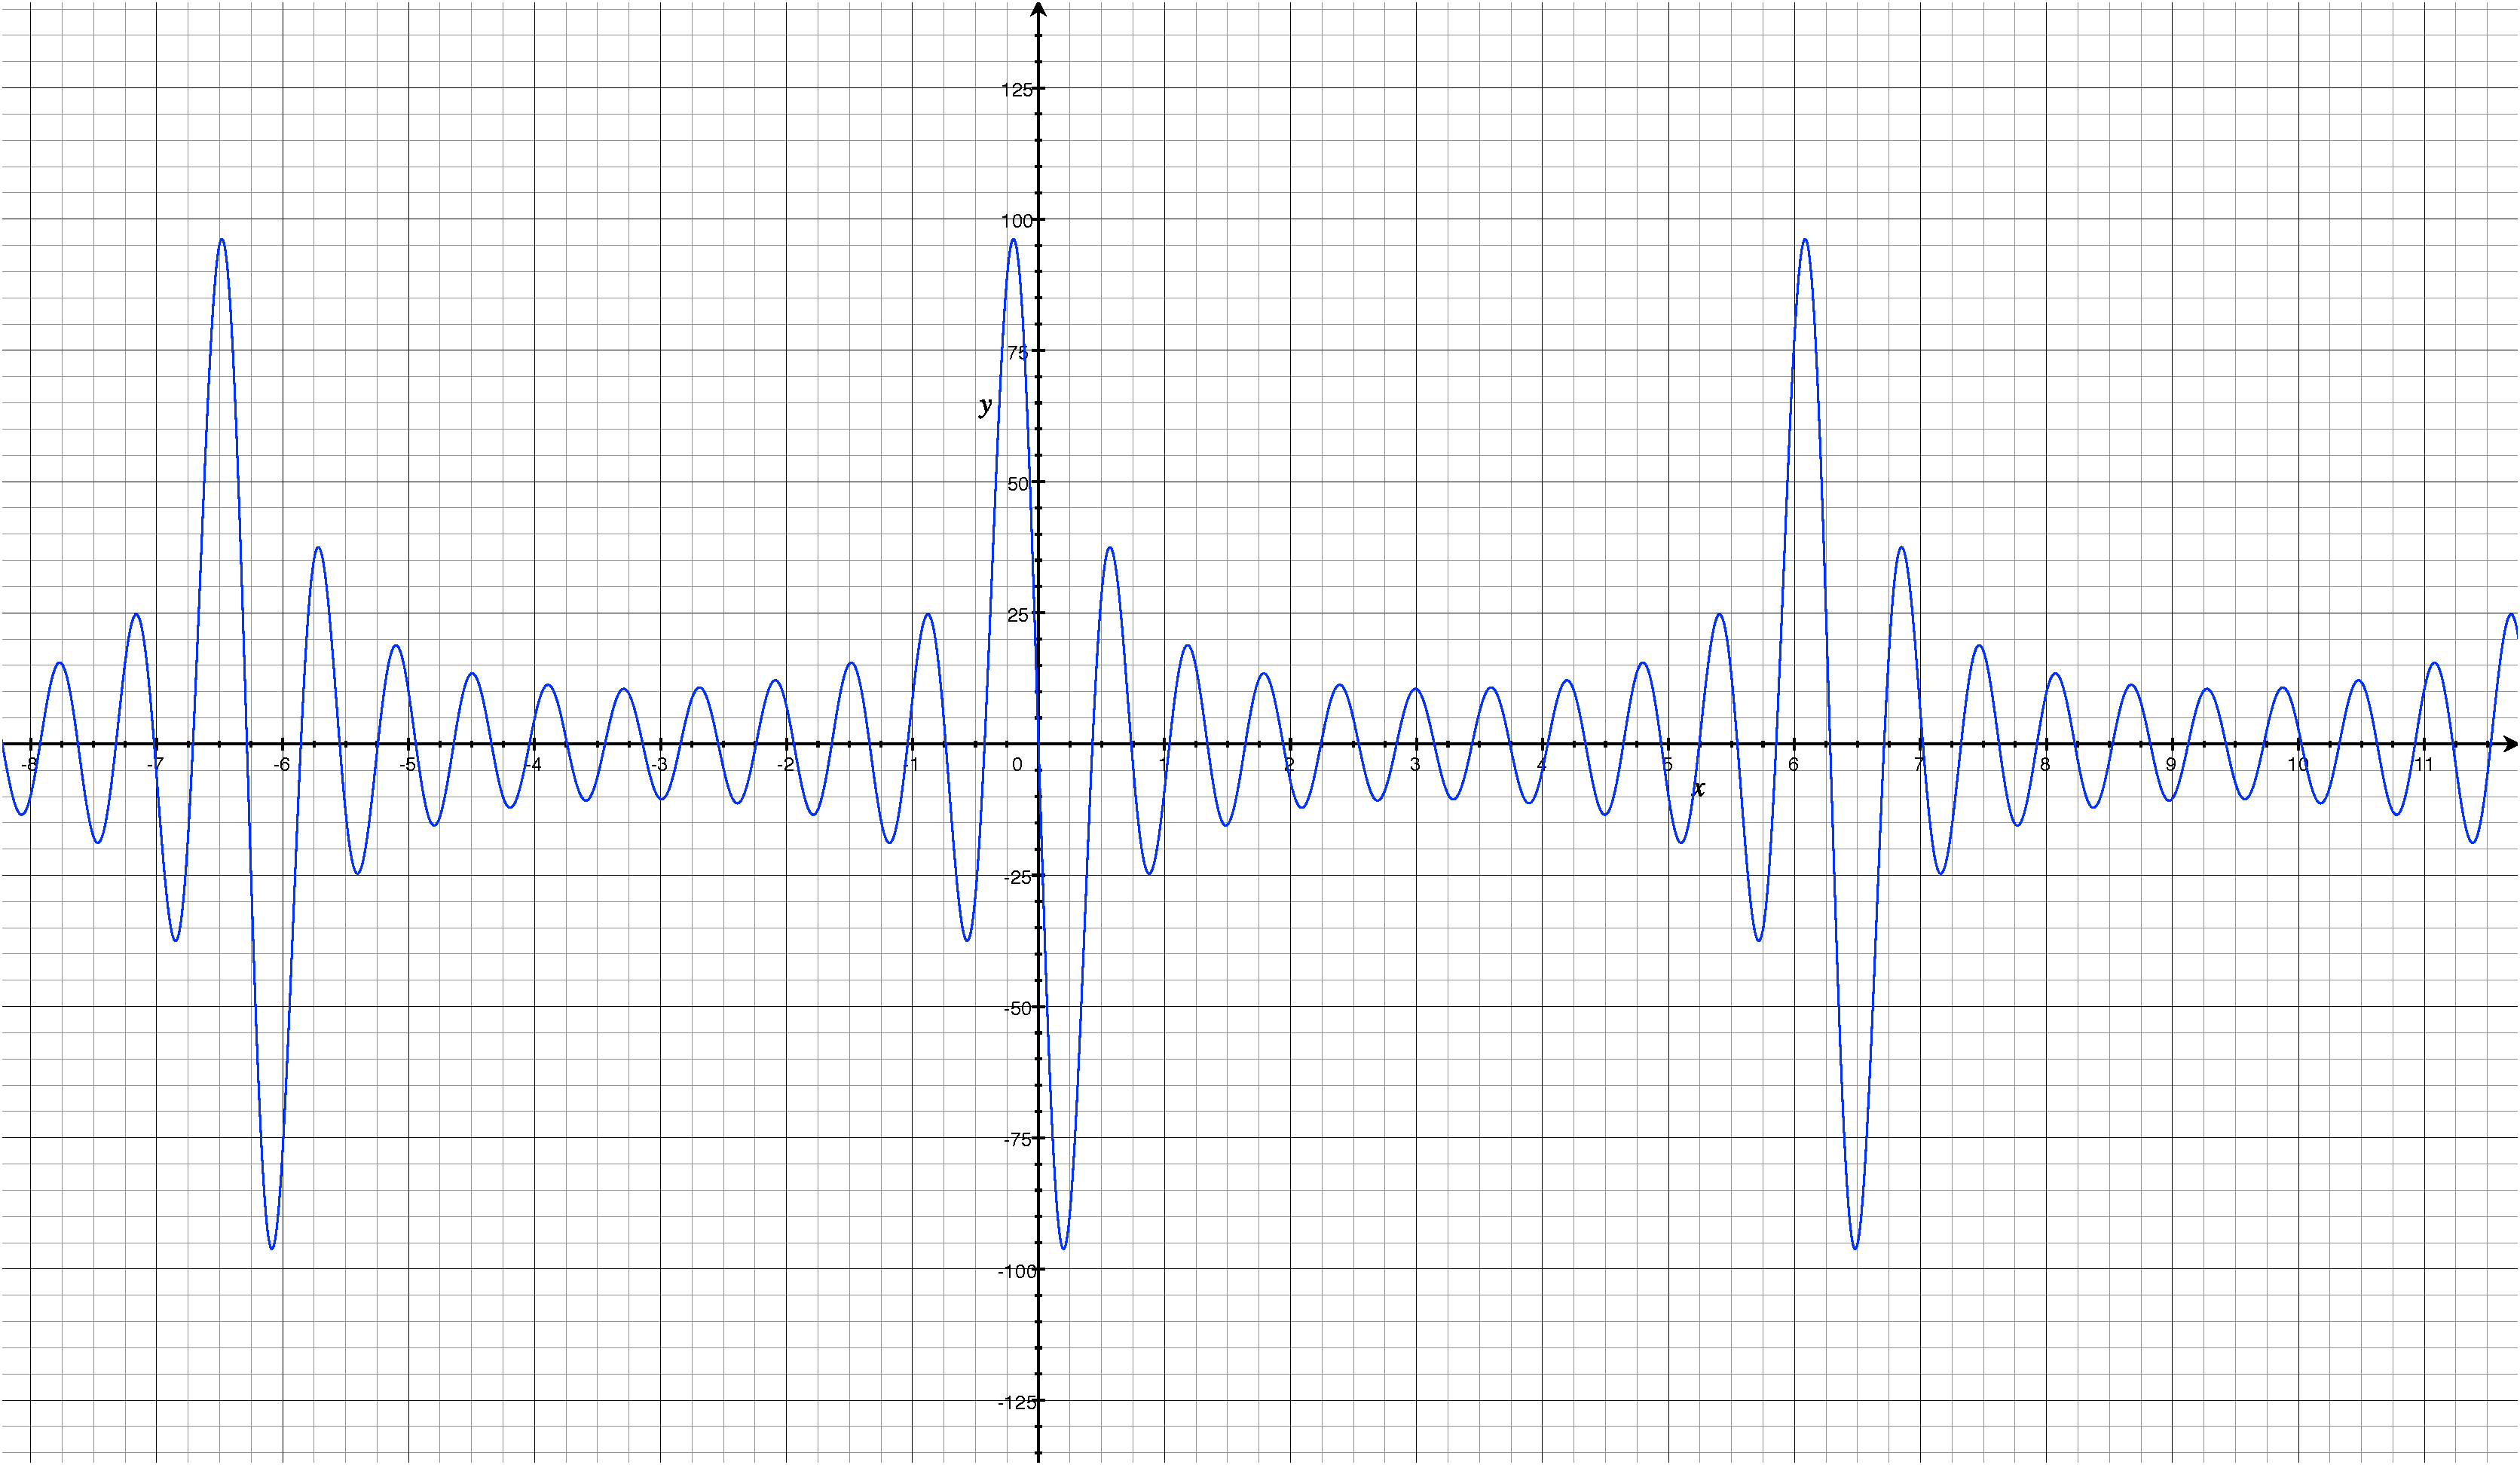
\includegraphics[width=1.0\textwidth]{Uebung3/Aufgabe_3_3_a_1.pdf} 
   \caption{$s(t)=\sum_{k=1}^n b_{k}sin(kt)=\sum_{k=1}^{n} jke^{jkt}-jke^{-jkt}, b_{k=-2k}, n=10$}
   \label{fig:3.3.a}
\end{figure}
\begin{figure}[p] %  figure placement: here, top, bottom, or page
   \centering
   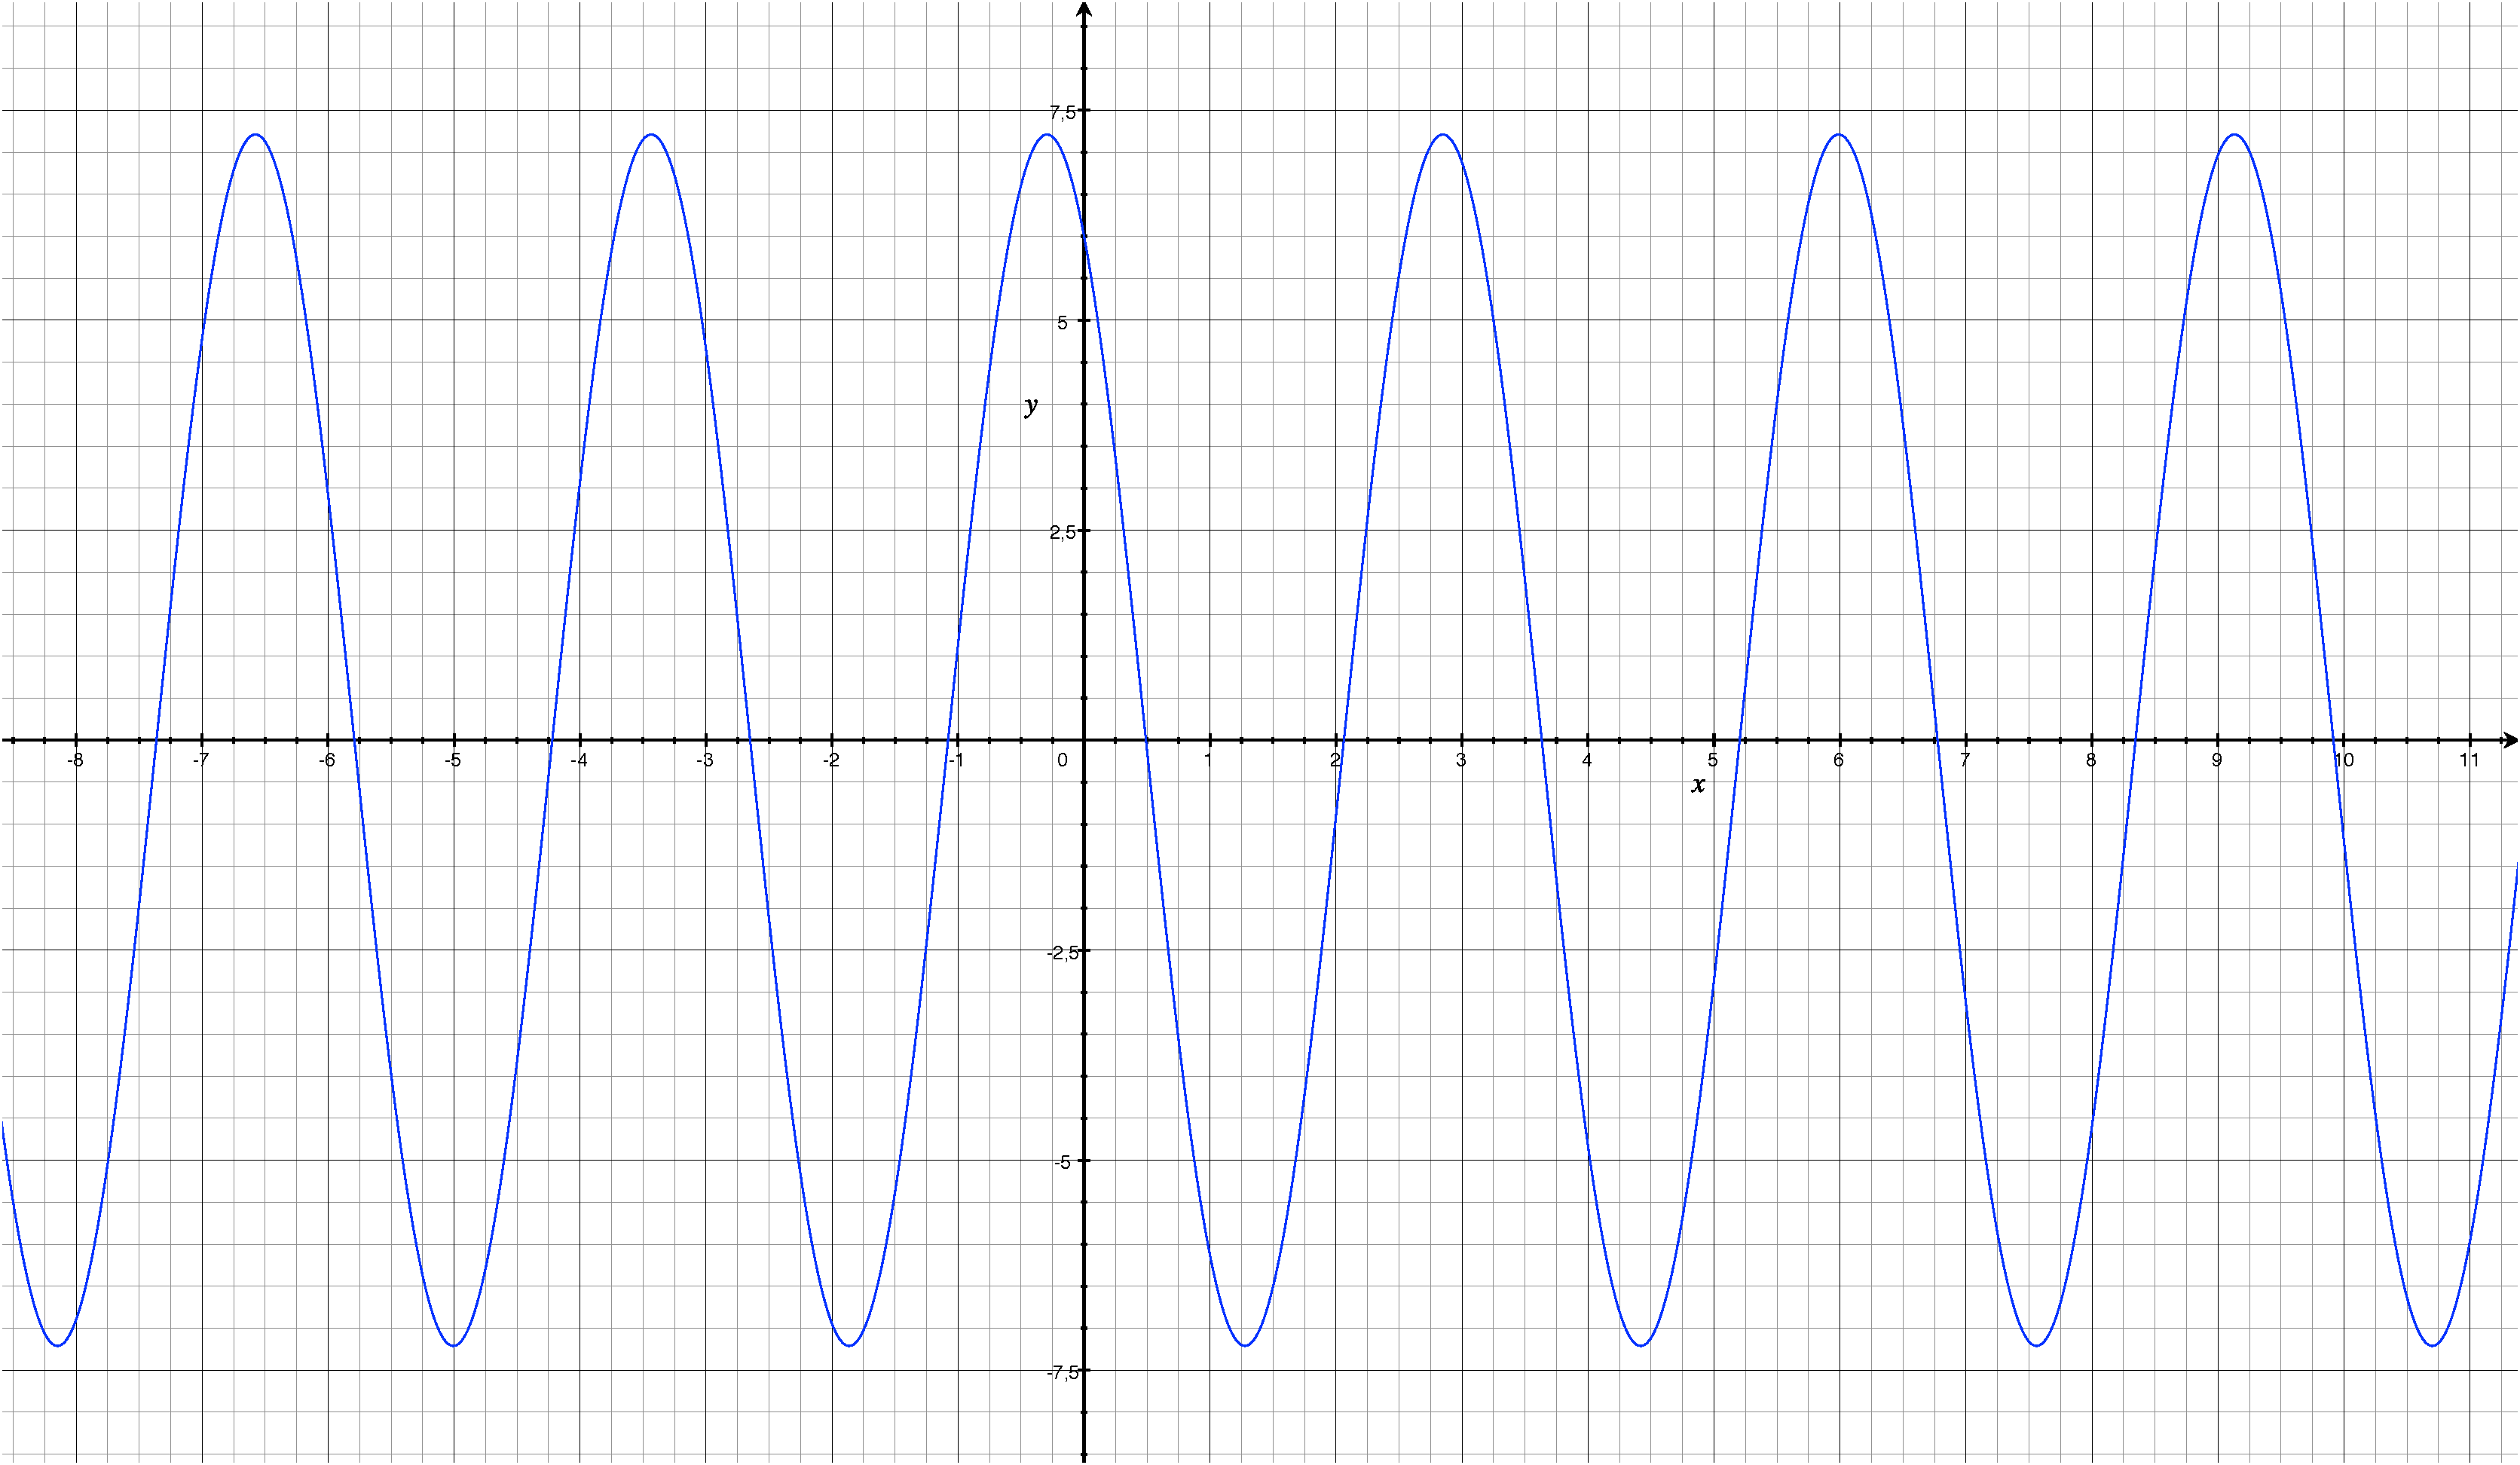
\includegraphics[width=1.0\textwidth]{Uebung3/Aufgabe_3_3_b.pdf} 
   \caption{$s(t)= 6cos(2t)-4sin(2t)=(3+2j)e^{j2t}+(3-2j)e^{-j2t}$}
   \label{fig:3.3.b}
\end{figure}
\end{document}